\documentclass[serif,xcolor=pdftex,dvipsnames,table,hyperref={bookmarks=false,breaklinks}]{beamer}

%%%%%%%%%%%%%%%%
% Change the macros below to configure the title slides
% for your course.
\newcommand{\coursename}{COMPSCI 589}
\newcommand{\instructor}{Benjamin M. Marlin}
\newcommand{\university}{University of Massachusetts Amherst}
\newcommand{\department}{College of Information and Computer Sciences}
%%%%%%%%%%%%%%%%


\newcommand{\settitlecard}[2]{
  \title[\coursename  Lecture #1] 
    {\coursename \\ Lecture #1: #2}
     \author[\instructor]{\instructor}
     \institute[\university]{
     \department\\
     \university
   }
\date{}
}

\newcommand{\maketitlepage}{
  \begin{frame}
  \titlepage
  \center{
    %If you use the slides unmodified, retain the attribution below
    \tiny{Slides by Benjamin M. Marlin (marlin@cs.umass.edu). \\
    \vspace{-1em}Created with support from National Science Foundation Award\# IIS-1350522. 
    %If you modify the slides, please retain the alternate attribution below
    %\tiny{Based on slides by Benjamin M. Marlin (marlin@cs.umass.edu). \\    
    %\vspace{-1em}Created with support from National Science Foundation Award\# IIS-1350522. 
    }                                              
  }  
  \end{frame}
}

\AtBeginSection[]
{
  \begin{frame}<beamer>{Outline}
    \tableofcontents[currentsection,subsectionstyle=hide]
  \end{frame}
}


\newcommand{\cut}[1]{}

\newcommand{\iconbox}[4]{
  \only<#1-#2>{
    \begin{columns}[T]
      \column{0.5in}
           \includegraphics[width=0.5in]{#3}
       \column{3.7in}
            #4
    \end{columns}
    \medskip
    \medskip
    \medskip
  }
}

\mode<presentation>{
  \usepackage{../beamertheme589theme}
  \setbeamercovered{invisible}
}

\mode<handout>{
  \usepackage{../beamertheme589theme}
  \setbeamercovered{transparent}
}


\usepackage[english]{babel}
\usepackage[latin1]{inputenc}
\usepackage{times}
\usepackage[T1]{fontenc}
\usepackage{amsmath}
\usepackage{amssymb}
\usepackage[noend]{algorithmic}
\usepackage{algorithm}
\usepackage{listings}

\renewcommand\mathfamilydefault{\rmdefault}

\newcommand{\setA}{\mathcal{A}}
\newcommand{\setB}{\mathcal{B}}
\newcommand{\setS}{\mathcal{S}}
\newcommand{\setV}{\mathcal{V}}
\DeclareMathOperator*{\union}{\bigcup}
\DeclareMathOperator*{\intersection}{\bigcap}
\DeclareMathOperator*{\Val}{Val}
\newcommand{\mbf}[1]{{\mathbf{#1}}}
\DeclareMathOperator*{\argmax}{arg\,max}
\DeclareMathOperator*{\argmin}{arg\,min}
\DeclareMathOperator*{\sign}{sign}
\newcommand{\deriv}[2]{\frac{\partial{#1}}{\partial{#2}}}


\settitlecard{1}{Course Overview - Supervised and Unsupervised Learning}

\begin{document}

\maketitlepage

\section{Introduction}
\subsection{Foo}


\begin{frame}[t]{Introduction}
  \center
  \Huge{What is Learning?}
\end{frame}

\begin{frame}[t]{Definitions of Learning}

\iconbox{1}{3}{../Figures/bfskinner.jpg}{\textbf{Behaviorism (Skinner, 1900-1950):} Learning is a long-term change in behavior due to experience.}

\iconbox{2}{3}{../Figures/gestalt.jpg}{\textbf{Cognitivism (Gestalt School, 1920-):} Learning is an internal mental process that integrates new information into established mental frameworks and updates those frameworks over time.}

\iconbox{3}{3}{../Figures/hebb.png}{\textbf{Connectionism (Hebb, 1949):} Learning is a physical process in which neurons join by developing the synapses between them.}

\end{frame}

\begin{frame}[t]{Introduction}
  \center
  \Huge{What is Machine Learning?}
\end{frame}

\begin{frame}[t]{Views on Machine Learning}

\iconbox{1}{2}{../Figures/samuel.jpg}{\textbf{Samuel (1959):} ``Machine learning is a field of study that gives computers the ability to learn without being explicitly programmed.''}

\iconbox{2}{2}{../Figures/mitchell.jpg}{\textbf{Mitchell (1997):} ``A computer program is said to learn from experience E with respect to some class of tasks T and performance measure P, if its performance at tasks in T, as measured by P, improves with experience E.''\\[12pt] \pause Substitute ``training data D'' for  ``experience E.''}



\end{frame}

\begin{frame}[t]{Machine Learning Tasks}
 \centering
 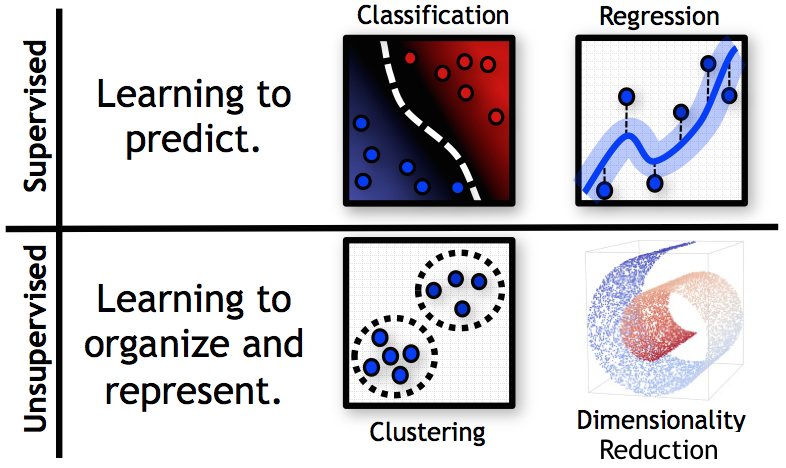
\includegraphics[width=4in]{../Figures/learning_problems.png}
\end{frame}

\begin{frame}[t]{Machine Learning Approaches}
  \begin{itemize}[<+->]
    \item \textbf{Non-Parametric:} Learning is accomplished by storing the training data (memorization).
    
    \item \textbf{Parametric:} Learning is accomplished by using an algorithm to adapt the parameters in a mathematical or statistical model given training data. For exmaple:\\
    
    \onslide<+->{\Large{ $$f_{\theta}(\mbf{x}) = \sum_{d=1}^D\theta_d x_d$$}}
    
  \end{itemize}
\end{frame}

\begin{frame}[t]{Machine Learning Applications}
 \centering
 
\includegraphics[width=4in]{../Figures/ml_applications.png}
\end{frame}

\begin{frame}[t]{Machine Learning in Industry}
 \centering
 
\includegraphics[width=4in]{../Figures/ml_industry.pdf}
\end{frame}


\begin{frame}[t]{Relationship to Other Fields}
  \begin{itemize}[<+->]
    \item Machine Learning and Artificial Intelligence
    \item Machine Learning and Probability/Statistics
    \item Machine Learning and Numerical Optimization
    \item Machine Learning and Function Approximation
    \item Machine Learning and Cognitive Science
    \item Machine Learning and Neuroscience
    \item Machine Learning and Data Mining 
    \item Machine Learning and Data Science
    \item Machine Learning and Big Data
  \end{itemize}
\end{frame}



\section{About the Course}
\subsection{Foo}

\begin{frame}[t]{Course Goals}

The aim of this course is to develop the knowledge and skills necessary to effectively apply existing machine learning models and algorithms to solve real-world problems. The course will cover:

\pause
\begin{itemize} [<+->]
\item Classification, regression, clustering, dimensionality reduction and representation learning 
\item Model selection, regularization, design of experiments, model evaluation
\item Use of machine learning across different computing contexts (desktop/cluster/cloud)
\end{itemize}

\onslide<+->{This course \textbf{will not} teach you how to design new machine learning models and
algorithms.}

\end{frame}

\begin{frame}[t]{Prerequisites}

The course has formal prerequisites as listed below. All students are expected to be familiar with this material or have the ability to make up any gaps in their backgrounds on their own.

\begin{itemize} [<+->]
\item Linear Algebra
\item Calculus
\item Probability and Statistics
\item Algorithms and Data Structures 
\end{itemize}

\onslide<+->{ The course requires the use of Python for programming. Students are expected to learn Python as we go.}

\end{frame}


\begin{frame}[t,label=current]{Text Books}

The course will use a two textbooks freely available from the authors:

\pause
\begin{itemize}[<+->]
\item {[ISL]}: \textit{An Introduction to Statistical Learning}. James, Witten, Hastie and Tibshirani.
\item {[ESL]}: \textit{The Elements of Statistical Learning, Second Edition}. Hastie, Tibshirani and Friedman.
\end{itemize}

\onslide<+->{Readings are intended to be completed before class.}

\end{frame}

\begin{frame}[t]{Programming and Computing}

\begin{itemize}[<+->]
\item Students need access to computing to complete regular assignments (any moderately recent laptop/desktop should do).
\item Programming assignments will use Python 2.7.
\item A complete Ubuntu programming environment will be distributed using Vagrant/Virtual Box. 
\item Access to cloud computing resources is required to complete course components using Apache Spark. 
\end{itemize}

\end{frame}

\section{Review and Notation}
\subsection{foo}

\begin{frame}[t]{Linear Algebra}

\begin{block}{Definition: Vector Space}
  The real vector space $\mathbb{R}^n$ is a set with elements  $\mbf{x}=[x_1,...,x_n]$
  where each $x_i \in \mathbb{R}$. The elements $\mbf{x}$ are called vectors, and they satisfy the following properties:
  
  \pause
  \begin{itemize}[<+->]
    \item \textbf{Addition:} If $\mbf{x}\in \mathbb{R}^n$ and $\mbf{y}\in \mathbb{R}^n$, then 
    $\mbf{x} + \mbf{y}=[x_1+y_1,...,x_n+y_n] \in \mathbb{R}^n$.
    \item \textbf{Scalar Product:} If $\mbf{x}\in \mathbb{R}^n$ and $a \in \mathbb{R}$, then 
    $a\mbf{x} =[ax_1,...,ay_n] \in \mathbb{R}^n$.
    \item \textbf{Inner Product:} If $\mbf{x}\in \mathbb{R}^n$ and $\mbf{y}\in \mathbb{R}^n$, then 
    $\mbf{x}\cdot\mbf{y} = \sum_{i=1}^n x_iy_i$.
  \end{itemize}

\end{block}
\end{frame}

\begin{frame}[t]{Linear Algebra}

\begin{block}{Definition: Matrix}
  A matrix $\mbf{X}\in \mathbb{R}^{n\times m}$ is rectangular array of elements $x_{ij}\in\mathbb{R}$, $1\leq i \leq n$, $1\leq j \leq m$:
  
  $$\mbf{X} =
 \begin{pmatrix}
  x_{11} & x_{12} & \cdots & x_{1m} \\
  x_{21} & x_{22} & \cdots & x_{2m} \\
  \vdots  & \vdots  & \ddots & \vdots  \\
  x_{n1} & x_{n2} & \cdots & x_{nm}
 \end{pmatrix}
  $$
  
\end{block}
\end{frame}

\begin{frame}[t]{Linear Algebra}

\begin{block}{Definition: Matrix}
  A matrix $\mbf{X}\in \mathbb{R}^{n\times m}$ supports the following operations:
  
  \pause
  \begin{itemize}[<+->]
    \item \textbf{Addition:} If $\mbf{X}\in \mathbb{R}^{n\times m}$, $\mbf{Y}\in \mathbb{R}^{n\times m}$ and $\mbf{Z}=\mbf{X}+\mbf{Y}$, then  $\mbf{Z}\in \mathbb{R}^{n\times m}$ and $Z_{ij}=X_{ij}+Y_{ij}$.

    \item \textbf{Scalar Product:} If $\mbf{X}\in \mathbb{R}^{n\times m}$, $a\in \mathbb{R}$
    and $\mbf{Z}=a\mbf{X}$, then  $\mbf{Z}\in \mathbb{R}^{n\times m}$ and $Z_{ij}=aX_{ij}$.
    
    \item \textbf{Matrix Product:} If $\mbf{X}\in \mathbb{R}^{n\times m}$, $\mbf{Y}\in \mathbb{R}^{m\times n}$ and $\mbf{Z}=\mbf{X}\mbf{Y}$, then  $\mbf{Z}\in \mathbb{R}^{n\times n}$ and $Z_{ij}=\sum_{k=1}^mX_{ik}Y_{kj}$.

  \end{itemize}  
\end{block}

\pause Yous should be familiar with basic matrix types (square, diagonal, identity), basic matrix operations (transpose, inverse, trace, determinant, etc.), and matrix concepts (eigenvalues, eigenvectors, orthogonality, etc.). 

\end{frame}


\begin{frame}[t]{Probability Distributions}

\begin{block}{Definition: Probability Distribution}

  A probability distribution $P$ over a sample space $\Omega$ is a mapping from subsets of $\Omega$ to the real numbers that satisfies the following conditions:

  \pause
  \begin{itemize}[<+->]
    \item Non-negativity: $P(\alpha) \geq 0$ for all $\alpha \subseteq \Omega$
    \item Normalization: $P(\Omega) =1$
    \item Additivity: For all $\alpha, \beta \subseteq  \Omega$ that are disjoint sets, $P(\alpha \union \beta) = P(\alpha) + P(\beta)$
  \end{itemize}

\end{block}
\end{frame}

\begin{frame}[t]{Random Variables} 
\begin{block}{Definition: Random Variable}
  A random variable $X$ is defined by a function $f_X$ that maps each element $\omega$ of the sample space $\Omega$ to a value $f_X(\omega)$ in a set $\mathcal{X}$ called the \emph{range} of the random variable.
  \medskip

  \pause
  For each $x\in \mathcal{X}$ the event $\{X=x\}$ refers to the subset of the sample space $\{\omega | \omega\in \Omega, f_X(\omega)=x\}$.
  \medskip
  
  \pause
  For each $x\in \mathcal{X}$ the probability $P(X=x) = P(\{\omega | \omega\in \Omega, f_X(\omega)=x\})$.
  
\end{block}
\end{frame}

\begin{frame}[t]{Probability and Random Variables} 
We can also specify a probability distribution for a random variable $X$ with range $\mathcal{X}$ directly instead of via an underlying sample space $\Omega$. The following conditions must hold:

\begin{itemize}[<+->]
\item \textbf{Discrete PMF:} $P(X=x)\geq 0 \;\;\forall x \in \mathcal X$ 
  and $\sum_{x\in\mathcal{X}}P(X=x)=1$.
\item \textbf{Continuous PDF:} $p(X=x)\geq 0 \;\; \forall x \in \mathcal X$ 
  and $\int_{\mathcal{X}}p(X=x)dx =1$.
\end{itemize}

\end{frame}


\begin{frame}[t]{Random Variables and Data Sets}

In machine learning and statistics, probability distributions are defined over data cases described by multiple attributes that are identified with random variables. 

 \pause 
 \begin{block}{Example: Heart Disease Dataset}
  \centering
  \rowcolors{2}{gray!25}{white}
  \begin{tabular}{cccc}
    \rowcolor{gray!50}
     Gender & Blood Pressure & Cholesterol  & Heart Disease\\
     Male&Med&Low&No\\
     Male&Hi&Hi&Yes\\
     Male&Med&Med&Yes\\
     Male&Med&Hi&No\\
     Female&Med&Low&No\\
     Male&Low&Med&No
  \end{tabular}
  \end{block}

\end{frame}



\begin{frame}[t]{Joint Probability Distributions}

\begin{itemize}
\item A \emph{joint probability distribution} is a probability distribution defined over a collection of random variables $(X_1,...,X_m)$ with ranges $\mathcal{X}_1,...,\mathcal{X}_m$: $P(X_1=x_1,...,X_m=x_m)$.

\pause
\item A joint distribution defined over random variables $X_1,...,X_m$ must satisfy normalization and non-negativity with respect to the Cartesian product of their ranges   $\mathcal{X}=\mathcal{X}_1\times \cdots \times \mathcal{X}_m$.

\pause
\item Alternatively, a joint distribution can be viewed as a probability distribution over a single vector-valued random variable $\mbf{X}=[X_1,...,X_m]$ whose range is $\mathcal{X}=\mathcal{X}_1\times \cdots \times \mathcal{X}_m$. 
\end{itemize}
\end{frame}


\begin{frame}[t]{Joint Distributions: Heart Disease Example}
Consider the heart disease example. The joint distribution over the random variables $Gender$, $BloodPressure$, $Cholesterol$ and $HeartDisease$ is just a big table:
\medskip 

  \pause
  \centering
  \rowcolors{2}{gray!25}{white}
  \begin{tabular}{ccccc}
    \rowcolor{gray!50}
      Gender & BloodPressure & Cholesterol  & HeartDisease & P\\
      F      & L       & L            & N             & 0.0127 \\
      F      & L       & L            & Y             & 0.0007 \\
      F      & L       & M            & N             & 0.0098 \\
      F      & L       & M            & Y             & 0.0009 \\
      F      & L       & H            & N             & 0.0087 \\
      F      & L       & H            & Y             & 0.0010 \\
     \vdots  & \vdots  & \vdots       & \vdots        & \vdots                
  \end{tabular}

\end{frame}



\begin{frame}[t]{Important Probability Concepts}

You should be familiar with the following fundamental concepts from probability theory

\pause
\begin{itemize}[<+->]
\item Marginalization
\item Conditioning
\item Bayes Rules
\item Expectations
\item Classical Distributions (Bernoulli, Binomial, Multinomial, Gaussian)
\end{itemize}

\end{frame}



\end{document}
